\part{Software Development}


\chapter{Model Building as Software Development}

\noindent
Developing a statistical model in Stan means writing a Stan program
and is thus a kind of software development process.  Developing
software is hard.  Very hard.  So many things can go wrong because
there are so many moving parts and combinations of parts.

Software development practices are designed to mitigate the problems
caused by the inherent complexity of writing computer programs.
Unfortunately, many methodologies veer off into dogma, bean counting,
or both.  A couple we can recommend that provide solid, practical
advice for developers are \citep{HuntThomas:99} and
\citep{McConnell:2004}.  This section tries to summarize some of their
advice.

\section{Use Version Control}

Version control software, such as Subversion or Git, should be in
place before starting to code.%
%
\footnote{Stan started using Subversion (SVN), then switched to the
  much more feature-rich Git package.  Git does everything SVN does
  and a whole lot more.  The price is a steeper learning curve.  For
  individual or very-small-team development, SVN is just fine.}
%
It may seem like a big investment to learn version control, but it's
well worth it to be able to type a single command to revert to a
previously working version or to get the difference between the
current version and an old version.  It's even better when you need
to share work with others, even on a paper---work can be done
independently and then automatically merged.  See
\refchapter{software-development} for information on how Stan itself
is developed.


\section{Make it Reproducible}

Rather than entering commands on the command-line when running models
(or entering commands directly into an interactive programming
language like R or Python), try writing scripts to run the data
through the models and produce whatever posterior analysis you need.
Scripts can be written for the shell, R, or Python.  Whatever language
a script is in, it should be self contained and not depend on global
variables having been set, other data being read in, etc.  

See \refchapter{reproducibility} for complete information on
reproducibility in Stan and its interfaces.

\subsection{Scripts are Good Documentation}

It may seem like overkill if running the project is only a single line
of code, but the script provides not only a way to run the code, but
also a form of concrete documentation for what is run. 


\subsection{Randomization and Saving Seeds}

Randomness defeats reproducibility.  MCMC methods are conceptually
randomized.  Stan's samplers involve random initializations as well as
randomization during each iteration (e.g., Hamiltonian Monte Carlo
generates a random momentum in each iteration).

Computers are deterministic.  There is no real randomness, just
pseudo-random number generators.  These operate by generating a
sequence of random numbers based on a ``seed.''  Stan (and other
languages like R) can use time-based methods to generate a seed based
on the time and date, or seeds can be provided to Stan (or R) in the
form of integers.  Stan writes out the seed used to generate the
data as well as the version number of the Stan software so that
results can be reproduced at a later date.%
%
\footnote{This also requires fixing compilers and hardware, because
  floating-point arithmetic does not have an absolutely fixed behavior
  across operating systems, hardware configurations, or compilers.}



\section{Make it Readable}

Treating programs and scripts like other forms of writing for an
audience provides an important perspective on how the code will be
used.  Not only might others want to read a program or model, the
developer will want to read it later.  One of the motivations of
Stan's design was to make models self-documenting in terms of variable
usage (e.g., data versus parameter), types (e.g., covariance matrix
vs. unconstrained matrix) and sizes.  

A large part of readability is consistency.  Particularly in naming
and layout.  Not only of programs themselves, but the directories and
files in which they're stored.

Readability of code is not just about comments (see
Section~\refsection{comments-programming} for commenting
recommendations and syntax in Stan).

It is surprising how often the solution to a debugging or design
problem occurs when trying to explain enough about the problem to
someone else to get help.  This can be on a mailing list, but it works
best person-to-person.  Finding the solution to your own problem when
explaining it to someone else happens so frequently in software
development that the listener is called a ``rubber ducky,'' because
they only have to nod along.%
%
\footnote{Research has shown an actual rubber ducky won't work.  For
  some reason, the rubber ducky must actually be capable of
  understanding the explanation.}


\section{Explore the Data}

Although this should go without saying, don't just fit data blindly.
Look at the data you actually have to understand its properties.  If
you're doing a logistic regression, is it separable?  If you're
building a multilevel model, do the basic outcomes vary by level?  If
you're fitting a linear regression, see whether such a model makes
sense by scatterplotting $x$ vs. $y$.

\section{Design Top-Down, Code Bottom-Up}

Software projects are almost always designed top-down from one or more
intended use cases.  Good software coding, on the other hand, is
typically done bottom-up.  

The motivation for top-down design is obvious.  The motivation for
bottom-up development is that it is much easier to develop software
using components that have been thoroughly tested.  Although Stan has
no built-in support for either modularity or testing, many of the same
principles apply.  

The way the developers of Stan themselves build models is to start as
simply as possibly, then build up. This is true even if we have a
complicated model in mind as the end goal, and even if we have a very
good idea of the model we eventually want to fit.  Rather than
building a hierarchical model with multiple interactions, covariance
priors, or other complicated structure, start simple.  Build just a
simple regression with fixed (and fairly tight) priors.  Then add
interactions or additional levels.  One at a time.  Make sure that
these do the right thing.  Then expand.

\section{Fit Simulated Data}

One of the best ways to make sure your model is doing the right thing
computationally is to generate simulated (i.e., ``fake'') data with
known parameter values, then see if the model can recover these
parameters from the data.  If not, there is very little hope that it
will do the right thing with data from the wild.  

There are fancier ways to do this, where you can do things like run
$\chi^2$ tests on marginal statistics or follow the paradigm
introduced in \citep{CookGelmanRubin:2006}, which involves interval
tests.  

\section{Debug by Print}

Although Stan does not have a stepwise debugger or any unit testing
framework in place, it does support the time-honored tradition of
debug-by-printf.%
%
\footnote{The ``f'' is not a typo --- it's a historical artifact of
  the name of the \code{printf} function used for formatted printing
  in C.} 

Stan supports print statements with one or more string or expression
arguments.  Because Stan is an imperative language, variables can have
different values at different points in the execution of a program.
Print statements can be invaluable for debugging, especially for a
language like Stan with no stepwise debugger.

For instance, to print the value of variables \code{y} and
\code{z}, use the following statement.
%
\begin{stancode}
print("y=", y, " z=", z);
\end{stancode}
%
This print statement prints the string ``y='' followed by the value of
\code{y}, followed by the string `` z=''
(with the leading space), followed by the value of the variable
\code{z}.

Each print statement is followed by a new line.  The specific ASCII
character(s) generated to create a new line are platform specific.

Arbitrary expressions can be used.  For example, the statement
\begin{stancode}
print("1+1=", 1+1);
\end{stancode}
%
will print ``1 + 1 = 2'' followed by a new line.

Print statements may be used anywhere other statements may be used,
but their behavior in terms of frequency depends on how often the
block they are in is evaluated.  See \refsection{print-statements} for
more information on the syntax and evaluation of print statements.



\section{Comments}\label{comments-programming.section}

\subsection{Code Never Lies}

The machine does what the code says, not what the documentation says.
Documentation, on the other hand, might not match the code.  Code
documentation easily rots as the code evolves if the documentation is
not well maintained.  

Thus it is always preferable to write readable code as opposed to
documenting unreadable code.  Every time you write a piece of
documentation, ask yourself if there's a way to write the code in such
a way as to make the documentation unnecessary.


\subsection{Comment Styles in Stan}

Stan supports \Cpp-style comments; see \refsection{comments} for full
details.  The recommended style is to use line-based comments for
short comments on the code or to comment out one or more
lines of code.  Bracketed comments are then reserved for long
documentation comments.  The reason for this convention is that
bracketed comments cannot be wrapped inside of bracketed comments.

\subsection{What Not to Comment}

When commenting code, it is usually safe to assume that you are 
writing the comments for other programmers who understand the basics 
of the programming language in use.  In other words, don't comment the
obvious.  For instance, there is no need to have comments
such as the following, which add nothing to the code.
%
\begin{stancode}
y ~ normal(0, 1);  // y has a unit normal distribution
\end{stancode}
%
A Jacobian adjustment for a hand-coded transform might be worth
commenting, as in the following example.
%
\begin{stancode}
exp(y) ~ normal(0, 1);
// adjust for change of vars: y = log | d/dy exp(y) |
target += y;
\end{stancode}
%
It's an art form to empathize with a future code reader and decide
what they will or won't know (or remember) about statistics and Stan.

\subsection{What to Comment}

It can help to document variable declarations if variables are given
generic names like \code{N}, \code{mu}, and \code{sigma}.  For
example, some data variable declarations in an item-response model
might be usefully commented as follows.
%
\begin{stancode}
int<lower=1> N;   // number of observations
int<lower=1> I;   // number of students
int<lower=1> J;   // number of test questions
\end{stancode}
%
The alternative is to use longer names that do not require comments.
%
\begin{stancode}
int<lower=1> n_obs;
int<lower=1> n_students;
int<lower=1> n_questions;
\end{stancode}
%
Both styles are reasonable and which one to adopt is mostly a matter of
taste (mostly because sometimes models come with their own naming
conventions which should be followed so as not to confuse readers of
the code familiar with the statistical conventions).

Some code authors like big blocks of comments at the top explaining
the purpose of the model, who wrote it, copyright and licensing
information, and so on.  The following bracketed comment is an
example of a conventional style for large comment blocks.
%
\begin{stancode}
/*
 * Item-Response Theory PL3 Model
 * -----------------------------------------------------
 * Copyright: Joe Schmoe  <joe@schmoe.com>
 * Date:  19 September 2012
 * License: GPLv3
 */

data {
  // ...
\end{stancode}
%
The use of leading asterisks helps readers understand the scope of the
comment.  The problem with including dates or other volatile
information in comments is that they can easily get out of synch with
the reality of the code.  A misleading comment or one that is wrong is
worse than no comment at all!



\chapter{Software Development Lifecycle}\label{software-development.chapter}

This chapter describes the software development lifecycle (SDLC) for
Stan, RStan, CmdStan, and PyStan. The layout and content very closely
follow the R regulatory compliance and validation document
\citep[Section~6]{RProject:2014}.

\section{Operational Overview}

The development, release, and maintenance of Stan is a collaborative
process involving the Stan development team.  The team covers multiple
statistical and computational disciplines and its members are based at
both academic institutions and industrial labs.

Communication among team members takes place in several venues.  Most
discussions take place openly on the Stan developers group, often
initiated by discussions in the Stan users group.%
%
\footnote{The groups are hosted by Google Groups, with information on
  reading and posting available from \url{http://mc-stan.org/groups.html}.}
%
The users and developers groups are archived and may be read by
anyone at any time. Communication that's not suitable for the public,
such as grant funding, is carried out on a private group restricted to
the core Stan developers. Further issue-specific discussion takes
place concurrently with development and source control.%
%
\footnote{The issue tracker for feature requests and bug reports is
  hosted by GitHub.  Full information on reading and making issue
  requests is available from \url{http://mc-stan.org/issues.html}.}
%
Bigger design issues and discussions that should be preserved take
place on the project Wiki.%
%
\footnote{The Wiki is hosted by GitHub; see
  \url{https://github.com/stan-dev/stan/wiki}.}

The developers host a weekly videoconference during which project
issues are discussed and prioritized.%
%
\footnote{The weekly meetings are hosted on Google+.  They are not
  recorded or stored.}
%
The developers also meet informally at their places of employment
(e.g., Columbia University) or at conferences and workshops when
multiple team members are in attendance.  The developers also host
meetups for the public in locations including London and New York.%
%
\footnote{These meetings are organized through
  \url{http://meetups.com}.  For example, meetings in New York are
  organized through \url{http://www.meetup.com/Stan-Users-NYC/}.}

The Stan project employs standard software development, code review,
and testing methodologies, as described on the project Wiki pages
and later in this chapter.

Stan's C++ library and the CmdStan interface are released under the
terms of the new (3 clause) BSD license, with two dependent libraries
(Boost and Eigen), released under compatible libraries. The R
interface RStan and Python interface PyStan are released under the
GPLv3 license. All of the code is hosted on public version control
repositories and may be reviewed at any time by all members of the
Stan community.  This allows continuous feedback for both coding
standards, functionality, and statistical accuracy.

The size of the Stan community is difficult to estimate reliably
because there are no sales transactions and Stan's version control
distribution system (GitHub) does not provide download statistics.
There are over 950 users subscribed to the users group, and a
conservative estimate would put the number of users in the thousands.
This substantial user base provides the means to do continuous reviews
of real-world performance in real settings. Unlike proprietary
software only available in binary form, Stan's open-source code base
allows users to provide feedback at the code level.

\section{Source Code Management}

The source code for Stan's C++ library, CmdStan, PyStan, and RStan is
managed in separate version-control libraries based on Git
\citep{Chacon:2014} and hosted by GitHub under the GitHub organization
stan-dev (\url{https://github.com/stan-dev}). Push access (i.e., the
ability to write to the repository) is restricted to core developers
and very closely managed. At the same time, any user may provide (and
many users have provided) pull requests with patches for the system
(which are treated as any other pull request and fully tested and code
reviewed). Because of Git's distributed nature, everyone who clones a
repository produces a full backup of the system and all past versions.

\begin{figure}
\begin{center}
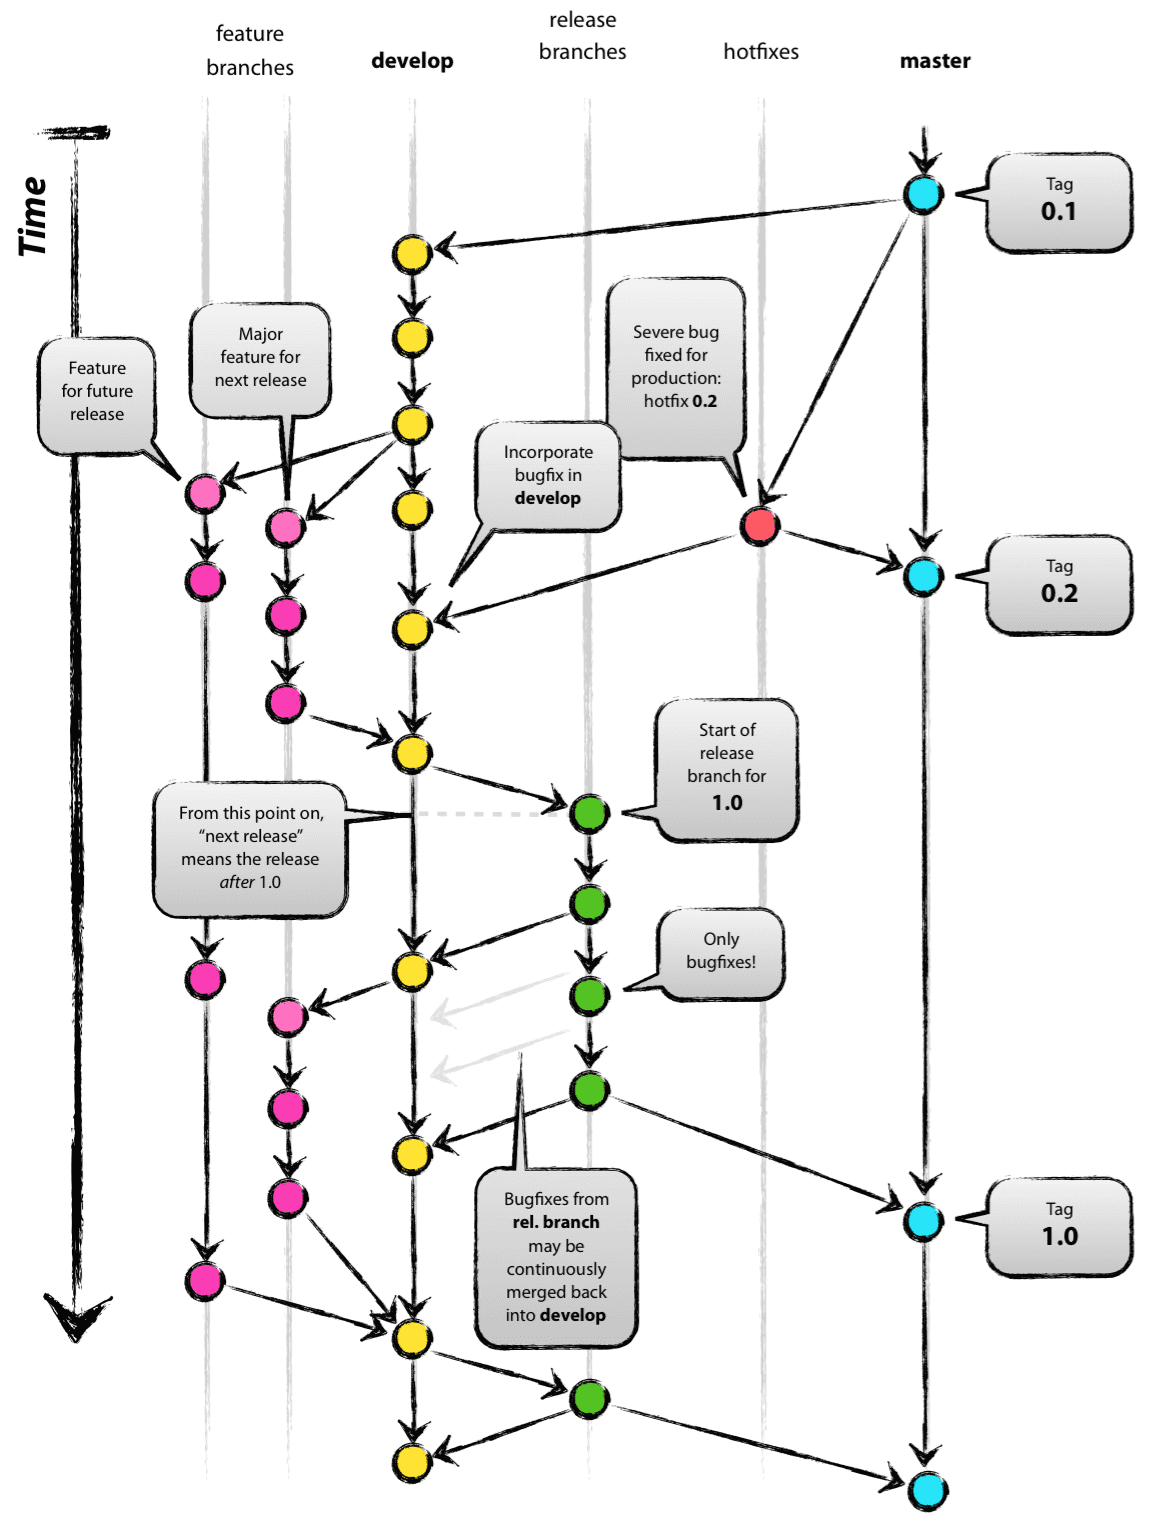
\includegraphics[height=4.5in]{img/git-process.png}
\end{center}
\caption{\small\it Git branching process for master
  and development branches.  New features and ordinary (not hot) 
  bugfixes are developed in branches from and merged back into the
  development  branch.  These are then
  collected into releases and merged with the master branch, which
  tracks the releases.  Hotfix branches are like feature or ordinary
  bugfix branches, but branch from master and merge back into master. 
  Image courtesy of \citep{Driessen:2010}.}\label{git-process.figure} \end{figure}
%
The basic Git process for branching, releasing, hotfixing, and merging
follows standard Git procedure \citep{Driessen:2010}. A diagram
outlining the process is presented in \reffigure{git-process}. The key
idea is that the master branch is always at the latest release, with
older commits tagged for previous releases. 

The development branch always represents the current state of
development. Feature and bugfix branches branch from the development
branch. Before being merged back into the development branch, they
must be wrapped in a pull request for GitHub, which supplies
differences with current code and a forum for code review and comment
on the issue. All branches must have appropriate unit tests and
documentation as part of their pull request before they will be merged
(see \url{https://github.com/stan-dev/stan/wiki/Pull-Request-Template}
for the pull request template which all requests must follow).  Each
pull request must provide a summary of the change, a detailed
description of the intended effect (often coupled with pointers to one
or more issues on the issue tracker and one or more Wiki pages), a
description of how the change was tested and its effects can be
verified, a description of any side effects, a description of any
user-facing documentation changes, and suggestions for reviewers.

Taken together, the testing, code review, and merge process ensures
that the development branch is always in a releasable state.

Git itself provides extensive log facilities for comparing changes
made in any given commit (which has a unique ID under Git) with any
other commit, including the current development or master branch.
GitHub provides further graphical facilities for commentary and
graphical differences.

For each release, the Git logs are scanned and a set of user-facing
release notes provided summarizing the changes. The full set of
changes, including differences with previous versions, is available
through Git.  These logs are complete back to the first version of
Stan, which was originally managed under the Subversion version
control system.

More information on the mechanics of the process are available from
on the Wiki page
\url{https://github.com/stan-dev/stan/wiki/Developer-Process}.

\section{Testing and Validation}

\subsection{Unit Testing}

Stan C++, CmdStan, PyStan, and RStan are all extensively unit tested.
The core C++ code and CmdStan code is tested directly in C++ using the
Google test framework \cite{GoogleTest:2011}. PyStan is tested using
the Python unit testing framework unittest%
%
\footnote{See \url{https://docs.python.org/3/library/unittest.html}.}
%
(formerly called ``PyTest'').  RStan is tested using the RUnit package.%
%
\footnote{See
  \url{http://cran.r-project.org/web/packages/RUnit/index.html}.}

The point of unit testing is to test the program at the application
programmer interface (API) level, not the end-to-end functional level.  

The tests are run automatically when pull requests are created through
a continuous integration process. PyStan uses the Travis continuous
integration framework;%
%
\footnote{See \url{https://travis-ci.org} for more on Travis.}
%
Stan C++ and CmdStan use Jenkins.%
%
\footnote{See \url{http://jenkins-ci.org} for more on Jenkins.}
%
The continuous integration servers provide detailed reports of the
various tests they run and whether they succeeded or failed.  If they
failed, console output is available pointing to the failed tests.  The
continuous integration servers also provide graphs and charts
summarizing ongoing and past testing behavior.

Stan and its interfaces' unit tests are all distributed with the
system software and may be run by users on their specific platform
with their specific compilers and configurations to provide support
for the reliability of a particular installation of Stan.

As with any statistical software, users need to be careful to consider
the appropriateness of the statistical model, the ability to fit it
with existing data, and its suitability to its intended application.

The entire source repository is available to users.  A snapshot at any
given release (or commit within a branch) may be downloaded as an
archive (zip file) or may be cloned for development under Git.
Cloning in Git provides a complete copy of all version history,
including every commit to every branch since the beginning of the
project.  

User feedback is accommodated through three channels. First, and most
formally, there is an issue tracker for each of Stan C++, CmdStan,
RStan and PyStan, which allows users to submit formal bug reports or
make feature requests.  Any user bug report is reviewed by the
development team, assessed for validity and reproducibility, and
assigned to a specific developer for a particular release target.
A second route for reporting bugs is our users group;  bugs reported
to the user group by users are then submitted to the issue tracker by
the developers and then put through the usual process.  A third method
of bug reporting is informal e-mail or comments; like the user group
reports, these are channeled through the issue tracker by the
developers before being tackled.

Continuous integration is run on a combination of Windows, Mac OS X,
and Linux platforms.  All core Stan C++ code is tested on Windows, Mac
OS, and Linux before release.


\subsection{Functional Testing}

In addition to unit testing at the individual function level, Stan
undergoes rigorous end-to-end testing of its model fitting
functionality. Models with known answers are evaluated for both speed
and accuracy. Models without analytic solutions are evaluated in terms
of MCMC error.  


\section{Release Cycles}

At various stages, typically when major new functionality has been
added or a serious bug has been fixed, the development branch is
declared ready for release by the Stan development team. At this
point, the branch is tested one last time on all platforms before
being merged with the master branch. Releases are managed through
GitHub releases mechanism.%
%
\footnote{For example, releases for Stan C++ are available on
\url{https://github.com/stan-dev/stan/releases}.}
%
Each release further bundles the manual and provides both a zipped and
tar-gzipped archive of the release.

Stan is released exclusively as source code, so nothing needs to be
done with respect to binary release management or compatibility.  The
source is tested so that it can be used under Windows, Mac OS X, and
Linux.  

Instructions for installing Stan C++, CmdStan, RStan, and PyStan are
managed separately and distributed with the associated product.

\section{Versioning and Release Compatibility}\label{version-numbering.section}

Stan version numbers follow the standard semantic version numbering
pattern in which version numbers are of the form
\code{Major.Minor.Patch}; for example version 2.9.1 is major release
2, minor release 9, and patch release 1.  Semantic versioning signals
important information about features and compatibiltiy for the Stan
language and how it is used.   It does not provide information about
underlying implementation;  changes in implementation do not affect
version numbering in and of itself.

See \refappendix{deprecated-features} for a list of currently
deprecated features and instructions on how to upgrade them.

\subsection{Major Version and Backward Compatiblity}

A change in a library breaks backward compatibility if a program that
worked in the previous version no longer works the same way in the
current version.  For backward-compatibility breaking changes, the
major version number is incremented.  When the major version is
updated, the minor version reverts to 0.  Because breaking backward
compatibility is such a disturbance for users, there are very few
major releases.

\subsection{Minor Version and Forward Compatibility}

A change in a library introduces a new feature if a program that works
in the current version will not work in a previous version; that is,
it breaks forward compatibility.  When a version introduces a new
feature without breaking backward compatibility, its minor version
number is incremented.  Whenever the minor version is incremented, the
patch level reverts to 0.  Most Stan releases increment the minor
version. 

\subsection{Bug Fixes and Patch Releases}

If a release does not add new functionality or break backward
compatibility, only its patch version is incremented.  Patch releases
of Stan are made when an important bug is fixed before any new work is
done.  Because Stan keeps its development branch clean, pending
patches are easily rolled into minor releases.

\section{Deprecating and Removing Features}\label{process-deprecation.section}

Before a user-facing feature is removed from software, it is polite to
deprecate it in order to maintain backward compatibility and provide
suggestions for upgrading.  \refappendix{deprecated-features} provides
a description of all of the deprecated features that are still
available in Stan and how to replace them with up-to-date features.

Eventually, deprecated features will be removed (aka retired).  As
explained in \refsection{version-numbering}, removing deprecated
features requires a major version number increment.  Stan 3.0.0 will
retire most if not all of the currently deprecated features.




\section{Availability of Current and Historical Archive Versions}

Current and older versions of Stan C++, CmdStan, RStan, and PyStan are
available through the GitHub pages for the corresponding repository.
Official releases are bundled as archives and available through
GitHub's releases (e.g.,
\url{https://github.com/stan-dev/stan/releases} for Stan C++).

Any intermediate commit is also available through GitHub in one of two
ways. First, all of Stan (or CmdStan, RStan, or PyStan) may be
downloaded by cloning the repository, at which point a user has a
complete record of the entire project's commits and branches. After
first cloning a repository, it may be kept up to date using Git's pull
command (available from the command-line or platform-specific
graphical user interfaces).   An alternative delivery mechanism is as
a zip archive of a snapshot of the system.  

\section{Maintenance, Support, and Retirement}

Stan support extends only to the most current release. Specifically,
patches are not backported to older versions.  

Early fixes of bugs are available to users in the form of updated
development branches. Snapshots of the entire code base at every
commit, including development patches and official releases, are
available from GitHub.  Git itself may be used to download a complete
clone of the entire source code history at any time.

There is extensive documentation in the form of manuals available for
the Stan language and algorithms
(\url{http://mc-stan.org/manual.html}), as well as each of the
interfaces, CmdStan (\url{http://mc-stan.org/cmdstan.html}), PyStan
(\url{http://mc-stan.org/pystan.html}), and RStan
(\url{http://mc-stan.org/cmdstan.html}). There is also an extensive
suite of example models (\url{http://mc-stan.org/documentation}) which
may be used directly or modified by users. There is also a fairly
extensive set of Wiki pages geared toward developers
(\url{https://github.com/stan-dev/stan/wiki}).

Issue trackers for reporting bugs and requesting features are
available online for Stan C++
(\url{https://github.com/stan-dev/stan/issues}), CmdStan
(\url{https://github.com/stan-dev/cmdstan/issues}), RStan
(\url{https://github.com/stan-dev/rstan/issues}), and PyStan
(\url{https://github.com/stan-dev/pystan/issues}).

There is Stan users group and also a group for Stan developers that
can be accessed online, in daily news digest form, or as an e-mail
list (see \url{http://mc-stan.org/groups.html}).  The users group is
where users can request support for installation issues, modeling
issues, or performance/accuracy issues.  These lists all come with
built-in search facilities through their host, Google Groups.

A number of books provide introductions to Stan, including {\it
  Bayesian Data Analysis, 3rd Edition} \citep{GelmanEtAl:2013} and
{\it Doing Bayesian Data Analysis, 2nd Edition} \citep{Kruschke:2014}.
All of the examples from two other books have been translated to
Stan, {\it Bayesian Cognitive Modeling: A Practical Course}
\citep{LeeWagenmakers:2013}, {\it The BUGS Book}
\citep{LunnEtAl:2012}, and {\it Data Analysis Using Regression and
  Multilevel-Hierarchical Models} \citep{GelmanHill:2007}.

The major.minor.0 releases are maintained through patch releases
major.minor.$n$ releases.  At each new major.minor.0 release, prior
versions are retired from support.  All efforts are focused on the
current release.  No further development or bug fixes are made
available for earlier versions.  The earlier versions can still be
accessed through version control.


\section{Qualified Personnel}

The members of the Stan development team are drawn from multiple
computational, scientific, and statistical disciplines across
academic, not-for-profit, and industrial laboratories. 

Most of Stan's developers have Ph.D. degrees, some have Master's
degrees, and some are currently enrolled as undergraduate or graduate
students. All of the developers with advanced degrees have published
extensively in peer reviewed journals. Several have written books on
statistics and/or computing. Many members of the core development team
were well known internationally outside of their contributions to Stan.
The group overall is widely acknowledged as leading experts in
statistical computing, software development, and applied statistics.

The managers of the development process have extensive industrial
programming experience and have designed or contributed to other
software systems that are still in production.

Institutions at which the members of the Stan development team hold
appointments as of Stan release 2.15.0 include Columbia University,
Adobe Creative Technologies Lab, University of Warwick, University of
Toronto (Scarborough), Dartmouth Colloge, University of Washington,
Lucidworks, CNRS (Paris), St. George's, University of London,
University of Massachussetts (Amherst), Aalto University, and Novartis
Pharma.

\section{Physical and Logical Security}

The Stan project maintains its integration servers for Stan C++ and
CmdStan on site at Columbia University. The integration servers for
Stan C++ and CmdStan are password protected and run on isolated,
standalone machines used only as integration servers. The network is
maintained by Columbia University's Information Technology (CUIT)
group.

The integration server for PyStan is hosted by the Travis open-source
continuous integration project, and is password protected on an
account basis.

The version control system is hosted by GitHub
(\url{http://github.com}). Due to Git's distributed nature, each
developer maintains a complete record of the entire project's commit
history. Everything is openly available, but privileges to modify the
existing branches is restricted to the core developers. Any change to
the code base is easily reversed through Git.

The archived releases as well as clones of the full repositories are
also managed through GitHub.

Stan's web pages are served by Pair, Inc. (\url{http://pair.com}) and
are password protected.  The web pages are purely informational and
nothing is distributed through the web page.

Individual contributors work on their own personal computers or on
compute clusters at Columbia or elsewhere.


\section{Disaster Recovery}

The entire history of the Stan C++, CmdStan, RStan, and PyStan
repositories is maintained on the GitHub servers as well as on each
developer's individual copy of the repository. Specifically, each
repository can be reconstituted from any of the core 
developers' machines.


\chapter{Reproducibility}\label{reproducibility.chapter}

\noindent
Floating point operations on modern computers are notoriously
difficult to replicate because the fundamental arithmetic operations,
right down to the IEEE 754 encoding level, are not fully specified.
The primary problem is that the precision of operations varies across
different hardware platforms and software implementations.

Stan is designed to allow full reproducibility.  However, this is only
possible up to the external constraints imposed by floating point
arithmetic.

Stan results will only be exactly reproducible if {\it all}\, of the following
components are {\it identical}\,:
%
\begin{itemize}
\item Stan version
\item Stan interface (RStan, PyStan, CmdStan) and version, plus version
  of interface language (R, Python, shell)
\item versions of included libraries (Boost and Eigen)
\item operating system version
\item computer hardware including CPU, motherboard and memory
\item \Cpp compiler, including version, compiler flags, and linked libraries
\item same configuration of call to Stan, including random seed, chain
  ID, initialization and data
\end{itemize}
%
It doesn't matter if you use a stable release version of Stan or the
version with a particular Git hash tag.  The same goes for all of the
interfaces, compilers, and so on.  The point is that if any of
these moving parts changes in some way, floating point results may
change.

Concretely, if you compile a single Stan program using the same
CmdStan code base, but changed the optimization flag (\code{-O3} vs.\
\code{-O2} or \code{-O0}), the two programs may not return the identical
stream of results.  Thus it is very hard to guarantee reproducibility
on externally managed hardware, like in a cluster or even a desktop
managed by an IT department or with automatic updates turned on.

If, however, you compiled a Stan program today using one set of flags,
took the computer away from the internet and didn't allow it to update
anything, then came back in a decade and recompiled the Stan program
in the same way, you should get the same results.

The data needs to be the same down to the bit level. For example, if
you are running in RStan, Rcpp handles the conversion between R's
floating point numbers and C++ doubles. If Rcpp changes the conversion
process or use different types, the results are not guaranteed to be
the same down to the bit level.  

The compiler and compiler settings can also be an issue.  There is a
nice discussion of the issues and how to control reproducibility in
Intel's proprietary compiler by \cite{CordenKreitzer:2014}.



\chapter{Contributed Modules}

\noindent
Stan is an open-source project and welcomes user contributions.  

In order to reduce maintenance on the main trunk of Stan development
and to allow developer-specified licenses, contributed Stan modules
are not distributed as part of Stan itself.


\section{Contributing a Stan Module}

Developers who have a Stan module to contribute should contact the
Stan developers either through one of the following.
%
\begin{itemize}
\item \code{stan-users} mailing list: 
\\
\url{https://groups.google.com/forum/?fromgroups#!forum/stan-users}
\item Stan e-mail: 
\\
\href{mailto:mc.stanislaw@gmail.com}{\tt mc.stanislaw@gmail.com}
\end{itemize}


\section{GitHub-Hosted Modules}

The \code{stan-dev} organization on GitHub hosts contributed projects
on GitHub.  This is also where the Stan developers will host works in
progress.  The full list of contributed projects on GitHub for
\code{stan-dev} is available at the following location.
%
\begin{quote}
\url{https://github.com/stan-dev}
\end{quote}

Each contributed module on \code{stan-dev}'s GitHub space comes with
its own documentation, indexed by the \code{README.md} file displayed
on GitHub.  Each contributed module has its own licensing the terms of
which are controlled by its developers.  The license for a contributed
package and its dependencies can be found in a top-level directory
\code{licenses/}.

\subsection{Emacs Stan Mode}

\noindent
Emacs Stan mode allows syntax highlighting and automatic indentation
of Stan models in the Emacs text editor.

\begin{quote}
\begin{tabular}{rl}
{\it Repository:} & \url{https://github.com/stan-dev/stan-mode}
\\[4pt]
{\it License:} & GPLv3
\\[4pt]
{\it Authors:} & Jeffrey Arnold, Daniel Lee
\end{tabular}
\end{quote}

\chapter{Stan Program Style Guide}

\noindent
This chapter describes the preferred style for laying out Stan
models. These are not rules of the language, but simply
recommendations for laying out programs in a text editor.  Although
these recommendations may seem arbitrary, they are similar to those of
many teams for many programming languages.  Like rules for typesetting
text, the goal is to achieve readability without wasting white space
either vertically or horizontally.

\section{Choose a Consistent Style}

The most important point of style is consistency.  Consistent coding
style makes it easier to read not only a single program, but multiple
programs.  So when departing from this style guide, the number one
recommendation is to do so consistently.

\section{Line Length}

Line lengths should not exceed 80 characters.%
%
\footnote{Even 80 characters may be too many for rendering in print;
  for instance, in this manual, the number of code characters that fit
  on a line is about 65.}
%
This is a typical recommendation for many programming language style
guides because it makes it easier to lay out text edit windows side by
side and to view the code on the web without wrapping, easier to view
diffs from version control, etc.  About the only thing that is
sacrificed is laying out expressions on a single line.

\section{File Extensions}

The recommended file extension for Stan model files is \code{.stan}.  
For Stan data dump files, the recommended extension is \code{.R}, or
more informatively, \code{.data.R}.

\section{Variable Naming}

The recommended variable naming is to follow C/\Cpp naming
conventions, in which variables are lowercase, with the underscore
character (\Verb|_|) used as a separator.  Thus it is preferred to use
\Verb|sigma_y|, rather than the run together \Verb|sigmay|, camel-case
\Verb|sigmaY|, or capitalized camel-case \Verb|SigmaY|.  Even matrix
variables should be lowercased.

The exception to the lowercasing recommendation, which also follows
the C/\Cpp conventions, is for size constants, for which the
recommended form is a single uppercase letter.  The reason for this is
that it allows the loop variables to match.  So loops over the indices of
an $M \times N$ matrix $a$ would look as follows.
%
\begin{stancode}
for (m in 1:M)
  for (n in 1:N)
     a[m,n] = ...
\end{stancode}


\section{Local Variable Scope}

Declaring local variables in the block in which they are used aids in
understanding programs because it cuts down on the amount of text
scanning or memory required to reunite the declaration and definition.

The following Stan program corresponds to a direct translation of a
BUGS model, which uses a different element of \code{mu} in each
iteration.
%
\begin{stancode}
model {
  real mu[N];
  for (n in 1:N) {
    mu[n] = alpha * x[n] + beta;
    y[n] ~ normal(mu[n],sigma);
  }
}
\end{stancode}
%
Because variables can be reused in Stan and because they should be
declared locally for clarity, this model should be recoded as follows.
%
\begin{stancode}
model {
  for (n in 1:N) {
    real mu;
    mu = alpha * x[n] + beta;
    y[n] ~ normal(mu,sigma);
  }
}
\end{stancode}
% 
The local variable can be eliminated altogether, as follows.
%
\begin{stancode}
model {
  for (n in 1:N)
    y[n] ~ normal(alpha * x[n] + beta, sigma);
}
\end{stancode}
%
There is unlikely to be any measurable efficiency difference
between the last two implementations, but both should be a bit
more efficient than the BUGS translation.

\subsubsection{Scope of Compound Structures with Componentwise Assignment}

In the case of local variables for compound structures, such as
arrays, vectors, or matrices, if they are built up component by
component rather than in large chunks, it can be more efficient to
declare a local variable for the structure outside of the block
in which it is used.  This allows it to be allocated once and then
reused.
%
\begin{stancode}
model {
  vector[K] mu;
  for (n in 1:N) {
    for (k in 1:K) 
      mu[k] = ...;
    y[n] ~ multi_normal(mu,Sigma);
}
\end{stancode}
%
In this case, the vector \code{mu} will be allocated
outside of both loops, and used a total of \code{N} times.

\section{Parentheses and Brackets}

\subsection{Optional Parentheses for Single-Statement Blocks}

Single-statement blocks can be rendered in one of two ways.  The fully
explicit bracketed way is as follows.
%
\begin{stancode}
for (n in 1:N) {
  y[n] ~ normal(mu,1);
}
\end{stancode}
%
The following statement without brackets has the same effect.
%
\begin{stancode}
for (n in 1:N)
  y[n] ~ normal(mu,1);
\end{stancode}
%  
Single-statement blocks can also be written on a single line, as
in the following example.
%
\begin{stancode}
for (n in 1:N) y[n] ~ normal(mu,1);
\end{stancode}
%
These can be much harder to read than the first example. Only use this
style if the statement is very simple, as in this example.  Unless
there are many similar cases, it's almost always clearer to put
each sampling statement on its own line.

Conditional and looping statements may also be written without brackets.

The use of for loops without brackets can be dangerous.  For instance,
consider this program.
%
\begin{stancode}
for (n in 1:N)
  z[n] ~ normal(nu,1);
  y[n] ~ normal(mu,1);
\end{stancode}
%
Because Stan ignores whitespace and the parser completes a statement
as eagerly as possible (just as in C++), the previous program is
equivalent to the following program.
%
\begin{stancode}
for (n in 1:N) {
  z[n] ~ normal(nu,1);
}
y[n] ~ normal(mu,1);
\end{stancode}
%


\subsection{Parentheses in Nested Operator Expressions}

The preferred style for operators minimizes parentheses.  This reduces
clutter in code that can actually make it harder to read expressions.
For example, the expression \code{a~+~b~*~c} is preferred to the
equivalent \code{a~+~(b~*~c)} or \code{(a~+~(b~*~c))}.  The operator
precedences and associativities are given in
\reffigure{operator-precedence}.

Similarly, comparison operators can usually be written with minimal
bracketing, with the form \code{y[n] > 0 || x[n] != 0} preferred to
the bracketed form \code{(y[n] > 0) || (x[n] != 0)}.  

\subsection{No Open Brackets on Own Line}

Vertical space is valuable as it controls how much of a program you
can see.  The preferred Stan style is as shown in the previous
section, not as follows.
%
\begin{stancode}
for (n in 1:N) 
{
  y[n] ~ normal(mu,1);
}
\end{stancode}
%
This also goes for parameters blocks, transformed data blocks, 
which should look as follows.
%
\begin{stancode}
transformed parameters {
  real sigma;
  ...
}
\end{stancode}
%


\section{Conditionals}

Stan supports the full \Cpp-style conditional syntax,
allowing real or integer values to act as conditions, as follows.
%
\begin{stancode}
real x;
...
if (x) {
   // executes if x not equal to 0
   ...
}
\end{stancode}
%

\subsection{Explicit Comparisons of Non-Boolean Conditions}

The preferred form is to write the condition out explicitly for
integer or real values that are not produced as the result of a
comparison or boolean operation, as follows.
%
\begin{stancode}
if (x != 0) ...
\end{stancode}


\section{Functions}

Functions are laid out the same way as in languages such as Java and
\Cpp.  For example,
%
\begin{stancode}
real foo(real x, real y) {
  return sqrt(x * log(y));
}
\end{stancode}
%
The return type is flush left, the parentheses for the arguments are
adjacent to the arguments and function name, and there is a space
after the comma for arguments after the first.  The open curly brace
for the body is on the same line as the function name, following the
layout of loops and conditionals.  The body itself is indented; here
we use two spaces.  The close curly brace appears on its own line.
%
If function names or argument lists are long, they can be
written as
%
\begin{stancode}
matrix
function_to_do_some_hairy_algebra(matrix thingamabob,
                                  vector doohickey2) {
  ...body...
}
\end{stancode}
%
The function starts a new line, under the type.  The arguments are
aligned under each other.

Function documentation should follow the Javadoc and Doxygen styles.
Here's an example repeated from \refsection{documenting-functions}.
%
\begin{stancode}
/**
 * Return a data matrix of specified size with rows 
 * corresponding to items and the first column filled 
 * with the value 1 to represent the intercept and the 
 * remaining columns randomly filled with unit-normal draws.
 *
 * @param N Number of rows correspond to data items
 * @param K Number of predictors, counting the intercept, per
 *          item.
 * @return Simulated predictor matrix.
 */
matrix predictors_rng(int N, int K) {  
  ...
\end{stancode}
%
The open comment is \code{/**}, asterisks are aligned below the first
asterisk of the open comment, and the end comment \code{*/} is also
aligned on the asterisk.  The tags \code{@param} and \code{@return}
are used to label function arguments (i.e., parameters) and return
values.  

\section{White Space}

Stan allows spaces between elements of a program.  The white space
characters allowed in Stan programs include the space (ASCII
\code{0x20}), line feed (ASCII \code{0x0A}), carriage return
(\code{0x0D}), and tab (\code{0x09}).  Stan treats all whitespace
characters interchangeably, with any sequence of whitespace characters
being syntactically equivalent to a single space character.
Nevertheless, effective use of whitespace is the key to good program
layout.


\subsection{Line Breaks Between Statements and Declarations}

It is dispreferred to have multiple statements or declarations on the
same line, as in the following example.
%
\begin{stancode}
transformed parameters {
  real mu_centered;  real sigma;
  mu = (mu_raw - mean_mu_raw);    sigma = pow(tau,-2);
}
\end{stancode}
%
These should be broken into four separate lines.

\subsection{No Tabs}

Stan programs should not contain tab characters.  They are legal and
may be used anywhere other whitespace occurs.  Using tabs to layout a
program is highly unportable because the number of spaces
represented by a single tab character varies depending on which
program is doing the rendering and how it is configured.  

\subsection{Two-Character Indents}

Stan has standardized on two space characters of indentation, which is
the standard convention for C/C++ code.  Another sensible choice is
four spaces, which is the convention for Java and Python.  Just be
consistent.  

\subsection{Space Between \code{if} and Condition}

Use a space after \code{if}s.  For instance, use \code{if (x < y) ...}, not
\code{if(x < y) ...}.

\subsection{No Space For Function Calls}

There is no space between a function name and the function it applies
to.  For instance, use \code{normal(0,1)}, not \code{normal (0,1)}.

\subsection{Spaces Around Operators}

There should be spaces around binary operators.  For instance, use
\code{y[1]~=~x}, not \code{y[1]=x}, use \code{(x~+~y)~*~z} not
\code{(x+y)*z}.

\subsection{Breaking Expressions across Lines}

Sometimes expressions are too long to fit on a single line.  In that
case, the recommended form is to break \emph{before} an operator,%
%
\footnote{This is the usual convention in both typesetting and other
  programming languages. Neither R nor BUGS allows breaks before an
  operator because they allow newlines to signal the end of an
  expression or statement.}
%
aligning the operator to indicate scoping.  For example, use the
following form (though not the content; inverting matrices is almost
always a bad idea).
%
\begin{stancode}
target += (y - mu)' * inv(Sigma) * (y - mu);
\end{stancode}
%
Here, the multiplication operator (\code{*}) is aligned to clearly
signal the multiplicands in the product.  

For function arguments, break after a comma and line the next
argument up underneath as follows.
%
\begin{stancode}
y[n] ~ normal(alpha + beta * x + gamma * y,
              pow(tau,-0.5));
\end{stancode}
%

\subsection{Optional Spaces after Commas}

Optionally use spaces after commas in function arguments for clarity.
For example, \code{normal(alpha * x[n] + beta,sigma)} can also be
written as \code{normal(alpha~*~x[n]~+~beta,~sigma)}.



\subsection{Unix Newlines}

Wherever possible, Stan programs should use a single line feed 
character to separate lines.  All of the Stan developers (so far, at 
least) work on Unix-like operating systems and using a standard 
newline makes the programs easier for us to read and share.  

\subsubsection{Platform Specificity of Newlines}

Newlines are signaled in Unix-like operating systems such as Linux and
Mac OS X with a single line-feed (LF) character (ASCII code point
\code{0x0A}).  Newlines are signaled in Windows using two characters,
a carriage return (CR) character (ASCII code point \code{0x0D})
followed by a line-feed (LF) character.
